\section{Acoustically-forced Transient Flame}\label{sec:oneDFlame}

The one-dimensional model of an acoustically-forced, freely-propagating premixed flame is now described. Similar constructions have been presented in prior work by the author and collaborators~\cite{Huang2022,Wentland2019}. The spatial domain is one-dimensional, spanning the length $x \in [0.0, \; 10]$ mm, subdivided into 1,024 cells of equal length. As with GEMS, a second-order Roe flux computes the inviscid fluxes, while gradients are computed by a central finite-difference stencil and limited by the face-oriented limiter of Barth and Jespersen.

The chemical system is composed of two fictitious species, a ``reactant'' species and a ``product'' species, having the calorically-perfect gas properties given in Table~\ref{tab:oneDFlameSpecs}. In this case, the fluid has a constant viscosity, unlike results in Section~\ref{sec:cavity} which computed viscosity via Sutherland's law. Note that the only difference between the two species is their enthalpy of formation. The reactant is converted to product by a single irreversible finite-rate reaction, governed by the Arrhenius parameters $A = 2.12 \times 10^{10}$ 1/s, $b = 0$, and $E_a = 2.025 \times 10^{8}$ kJ/mol.

\begin{table}
	\centering
	\begin{tabular}{ lllllll }
	\toprule
	Species & MW (g/mol) & $\cpSpec$ (kJ/kg-K) & $\refEnthSpec$ (kJ/kg) & $\dynViscSpec$ (kg/m-s) & $\prandtlSpec$ & $\schmidtSpec$   \\
	\midrule
	Reactant & 21.32 & 1.538 & -7,4320 & 7.35e-4 & 0.713 & 0.62 \\
	Product & 21.32 & 1.538 & -10,800 & 7.35e-4 & 0.713 & 0.62 \\
	\bottomrule
	\end{tabular}
	\caption{\label{tab:oneDFlameSpecs}Constant thermodynamic and transport properties of fictitious species.}
\end{table}

To begin, the solution is initialized with 100\% reactant at 300 K in the region $x \in [0.0, \; 0.02]$ mm, and the remainder of the domain is initialized with product at 2,400 K. The full domain is initialized with a pressure of 1 MPa and zero velocity. An approximate characteristic boundary condition is enforced at the outlet, and a fixed velocity is enforced at the inlet. Using BDF2 integration with a time step of 50 ns, the simulation is started with a velocity of 1 m/s at the inlet, which is manually adjusted until the flame is determined to be suitably ``stationary,'' balancing the bulk advection downstream with the reaction/diffusion upstream. At this point, 10 m/s is added to the velocity throughout the domain, and the primitive state appears as shown in Fig.~\ref{fig:flameIC}. This is the initial condition from which all further FOM simulations are computed. Further, for all further simulations (ROM or FOM), the inlet boundary condition is changed to an approximate characteristic boundary condition.

\begin{figure}
	\begin{minipage}{0.49\linewidth}
		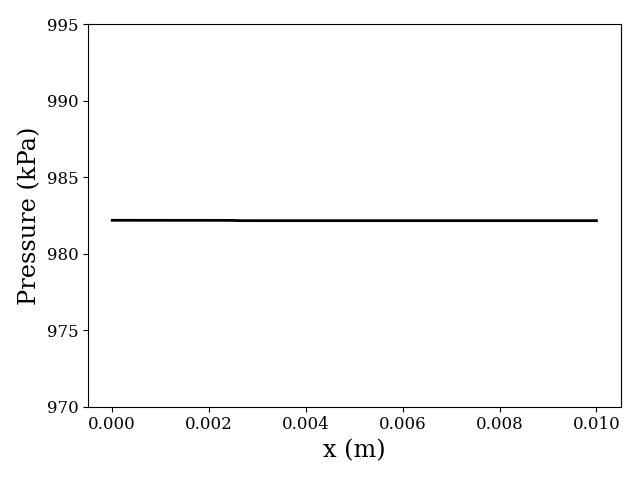
\includegraphics[width=0.99\linewidth]{Chapters/TransientFlame/Images/init_cond_pressure.png}
	\end{minipage}
	\begin{minipage}{0.49\linewidth}
		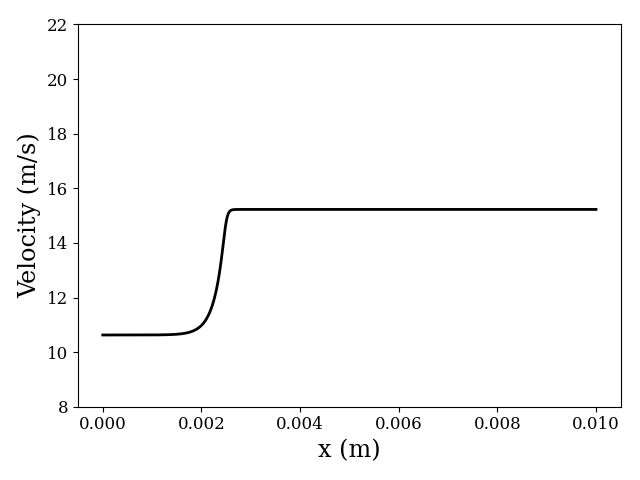
\includegraphics[width=0.99\linewidth]{Chapters/TransientFlame/Images/init_cond_vel.png}
	\end{minipage}

	\begin{minipage}{0.49\linewidth}
		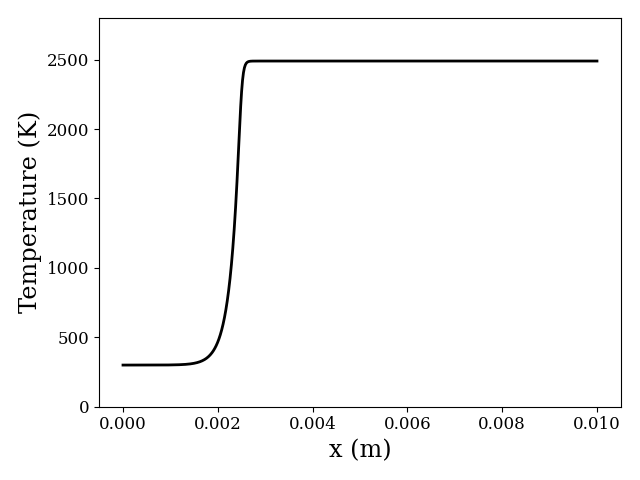
\includegraphics[width=0.99\linewidth]{Chapters/TransientFlame/Images/init_cond_temp.png}
	\end{minipage}
	\begin{minipage}{0.49\linewidth}
		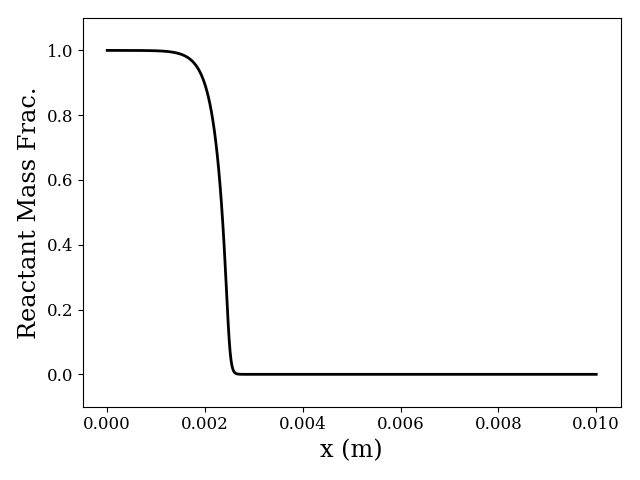
\includegraphics[width=0.99\linewidth]{Chapters/TransientFlame/Images/init_cond_mf.png}
	\end{minipage}
	\caption{\label{fig:flameIC}Initial condition for propagating flame FOM simulations.}
\end{figure}

To build a dataset of parametrically-varied simulations, an artificial pressure forcing is introduced to the outlet boundary condition. This forcing is computed as a sinusoidal perturbation about the outlet mean-flow pressure, of the form
%
\begin{equation}
	\pressureBack = \pressureMean \left[1 + A \; sin\left(2 \pi f \timeVar\right)\right]
\end{equation}
%
where $\pressureMean$ is the outlet mean-flow pressure (approximately 965 kPa in this case), $A$ is the percentage amplitude, and $f$ is the forcing frequency.